\chapter{Penglihatan dan Otak}\label{ch:g11:vision-and-brain}

Setelah sebuah stroke, seorang pasien melihat dunianya dengan sempurna
--- dalam hitam, putih dan kelabu. Pasien lain melihat warna dan bentuk
tetapi tanpa gerakan: sebuah mobil ada di sini, lalu di sana, tanpa apa
pun di antaranya, dan menuang teh menjadi mustahil karena
alirannya tidak pernah tampak bergerak. Pasien ketiga tidak dapat
mengenali wajah, termasuk wajahnya sendiri di cermin, walaupun ia
melukiskan tiap ciri wajahnya. \omterm{def:g11:the-eye:parts}{Mata} ketiganya utuh. Yang hilang dari
masing-masing adalah satu keping otak tempat melihat disusun. Bab ini
mengikuti saraf optik ke dalam otak, memetakan apa yang diperbuat
\omterm{prop:g11:vision-and-brain:pathway}{korteks penglihatan} dengan isyarat retinanya, dan menunjukkan bahwa
petanya tidak tetap: peta itu dibangun pengalaman, diubah pembelajaran,
dan diganggu obat.

\section{Dari retina ke korteksnya}

\begin{proposition}[Jalur penglihatannya]\label{prop:g11:vision-and-brain:pathway}
Sejuta serabut tiap saraf optiknya berjalan ke belakang menuju
\emph{kiasma optik}, tempat serabut dari separuh hidung tiap retinanya
menyeberang ke sisi yang lain sedangkan serabut dari separuh pelipisnya
tinggal pada sisinya sendiri. Di seberang kiasmanya, karena itu tiap
\emph{lajur optik} membawa isyarat dari separuh kiri kedua retinanya
(lajur kanan) atau dari separuh kanannya (lajur kiri) --- yaitu segala yang terlihat
pada separuh medan penglihatannya. Lajurnya beralih di \emph{talamus}
dan mencapai \emph{korteks penglihatan primer}\index{korteks
penglihatan}, di belakang tiap belahan otaknya: belahan kirinya
menerima separuh kanan medan penglihatannya, belahan kanannya separuh
kirinya.
\end{proposition}
\begin{proof}[Bukti percobaan]
Memotong satu saraf optik membutakan satu \omterm{def:g11:the-eye:parts}{mata}; kerusakan pada satu
lajur optik, atau pada \omterm{prop:g11:vision-and-brain:pathway}{korteks penglihatan} satu belahan otaknya,
membiarkan kedua \omterm{def:g11:the-eye:parts}{matanya} bekerja tetapi membutakan keduanya terhadap
separuh dunia yang sama --- yaitu separuh yang berlawanan dengan
lukanya. Merangsang satu titik \omterm{prop:g11:vision-and-brain:pathway}{korteks penglihatan} seorang pasien yang
sadar selama pembedahan membuatnya melihat kilatan pada kedudukan tetap
dalam medannya; titik yang bertetangga memberi kilatan yang
bertetangga: korteksnya memuat sebuah peta retinanya, dengan pusat
medannya menempati bagian yang terbesar.
\end{proof}

\begin{omfigure}
\begin{tikzpicture}[font=\small, >=Stealth, line cap=round]
  % top view: eyes at top, cortex at bottom
  \draw[thick, fill=omDef!8] (-2.2,4.2) circle (0.6); \draw[thick, fill=omDef!8] (2.2,4.2) circle (0.6);
  \node[anchor=south] at (-2.2,4.9) {mata kiri}; \node[anchor=south] at (2.2,4.9) {mata kanan};
  % visual field halves
  \node[omThm, anchor=east] at (-3.2,5.9) {medan kiri};
  \node[omMeth!60!black, anchor=west] at (3.2,5.9) {medan kanan};
  \draw[omThm, thick] (-4.4,5.6) -- (0,5.6); \draw[omMeth!60!black, thick] (0,5.6) -- (4.4,5.6);
  % fibres: left field falls on right halves of both retinas -> right hemisphere
  % from left eye: temporal half (left side of left eye) sees right field -> stays left; nasal half sees left field -> crosses
  \draw[thick, omMeth!60!black] (-2.7,3.7) -- (-2.7,1.6) -- (-1.2,0.3) -- (-1.2,-1.4);
  \draw[thick, omThm] (-1.7,3.7) -- (-1.7,1.6) -- (1.2,0.3) -- (1.2,-1.4);
  \draw[thick, omThm] (2.7,3.7) -- (2.7,1.6) -- (1.2,0.3);
  \draw[thick, omMeth!60!black] (1.7,3.7) -- (1.7,1.6) -- (-1.2,0.3);
  \fill (0,0.85) circle (2pt); \node[anchor=north] at (0,0.4) {kiasma optik};
  % thalamus relays
  \draw[thick, fill=gray!20] (-1.2,-0.4) ellipse (0.35 and 0.25); \draw[thick, fill=gray!20] (1.2,-0.4) ellipse (0.35 and 0.25);
  \node[anchor=east] at (-1.6,-0.4) {talamus};
  % cortex
  \draw[thick, fill=omMeth!15] (-2.4,-2.6) rectangle (-0.2,-1.4); \draw[thick, fill=omThm!15] (0.2,-2.6) rectangle (2.4,-1.4);
  \node[align=center] at (-1.3,-2.0) {korteks penglihatan\\ kiri}; \node[align=center] at (1.3,-2.0) {korteks penglihatan\\ kanan};
  \node[anchor=north, align=center, font=\scriptsize] at (-1.3,-2.7) {melihat\\ medan kanan};
  \node[anchor=north, align=center, font=\scriptsize] at (1.3,-2.7) {melihat\\ medan kiri};
  \node[anchor=west, align=left, font=\scriptsize] at (3.0,2.6) {saraf optik:\\ satu tiap mata};
  \node[anchor=west, align=left, font=\scriptsize] at (3.0,0.0) {lajur optik:\\ satu tiap separuh medan};
\end{tikzpicture}

{\small Jalur penglihatannya dilihat dari atas. Cahaya dari separuh
kiri medannya (merah) jatuh pada separuh kanan tiap retinanya;
serabutnya, yang menyeberang di kiasmanya bila perlu, berkumpul menjadi
lajur optik kanan dan mencapai \omterm{prop:g11:vision-and-brain:pathway}{korteks penglihatan} kanan. Tiap belahan
otaknya melihat separuh dunia yang berlawanan dengan kedua \omterm{def:g11:the-eye:parts}{matanya}.}
\end{omfigure}

\begin{omfigure}
\begin{tikzpicture}
  \node[anchor=south west, inner sep=0] (img) at (0,0)
    {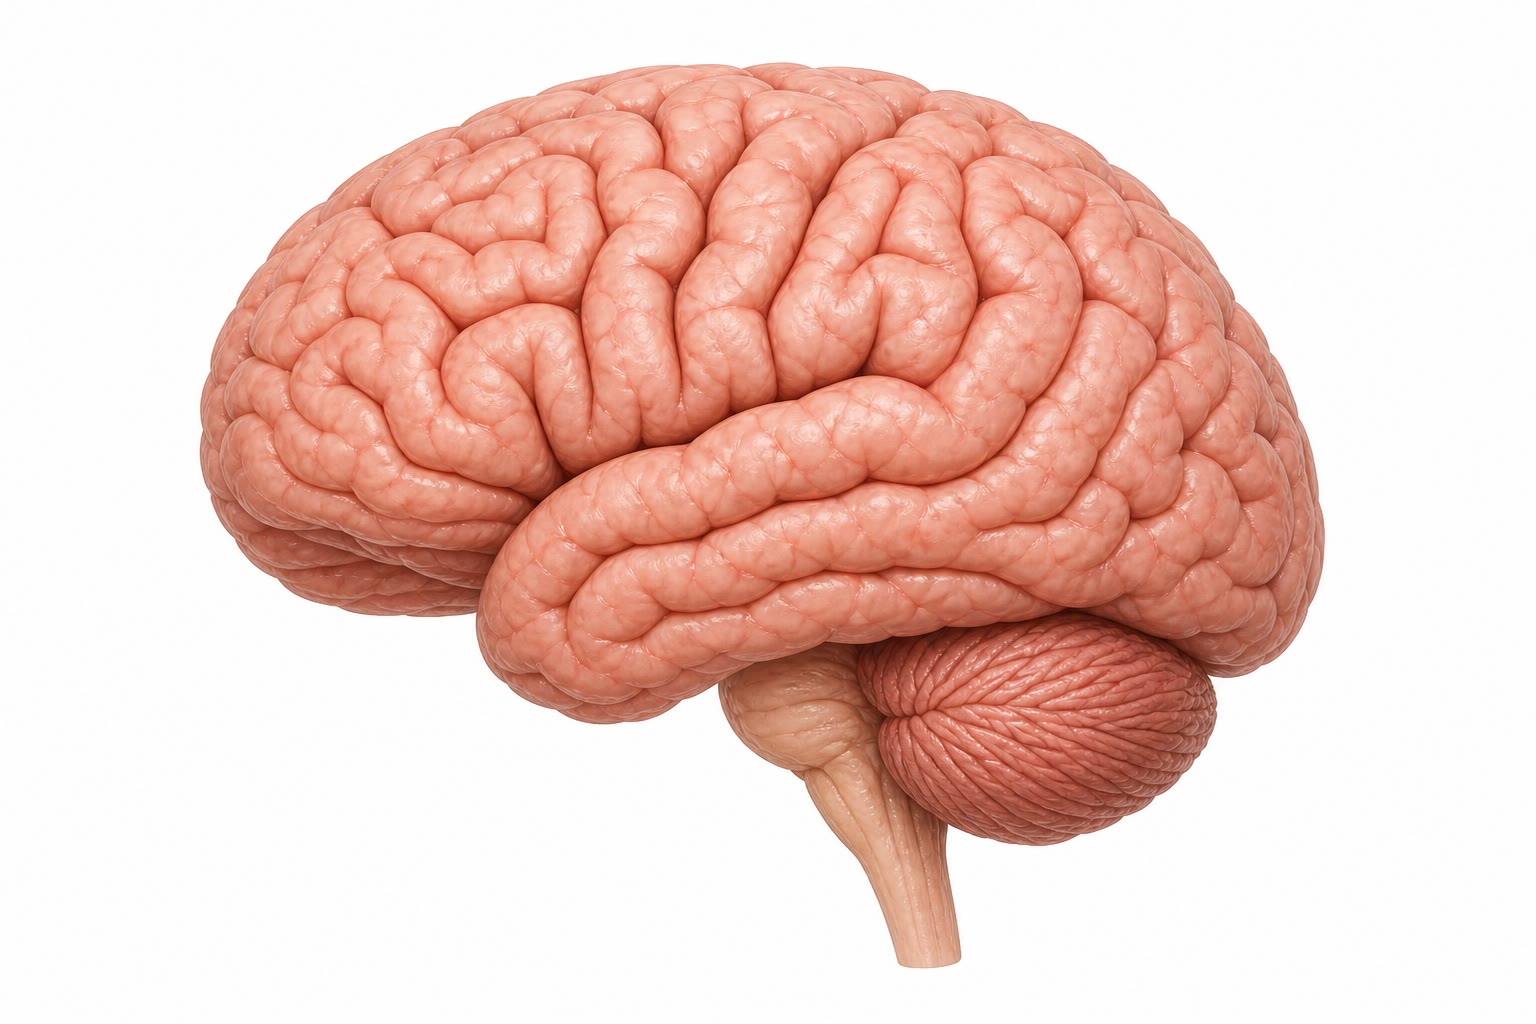
\includegraphics[width=0.52\linewidth]{images/book2/ai/fig-brain-side.jpg}};
  \begin{scope}[x={(img.south east)}, y={(img.north west)},
      every node/.style={font=\small}]
    \draw[omDef, thick] (0.85,0.55) -- (1.05,0.70) node[right, align=left] {korteks penglihatan primer\\ (lobus oksipital)};
    \draw[omDef, thick] (0.70,0.75) -- (0.80,1.06) node[above] {lobus parietal};
    \draw[omDef, thick] (0.28,0.72) -- (0.20,1.06) node[above] {lobus frontal};
    \draw[omDef, thick] (0.48,0.42) -- (0.40,-0.06) node[below] {lobus temporal};
    \draw[omDef, thick] (0.70,0.28) -- (1.05,0.20) node[right] {otak kecil};
  \end{scope}
\end{tikzpicture}

{\small Otak dilihat dari sisi kiri. \omterm{prop:g11:vision-and-brain:pathway}{Korteks penglihatan primernya}
terletak paling belakang, dalam lobus oksipitalnya; daerah penglihatan
selanjutnya membentang maju darinya ke dalam lobus temporal (benda itu
apa) dan lobus parietal (di mana benda itu dan bagaimana ia bergerak).}
\end{omfigure}

\section{Banyak daerah, satu tanggapan}

\begin{proposition}[Daerah penglihatan yang khusus]\label{prop:g11:vision-and-brain:areas}
\omterm{prop:g11:vision-and-brain:pathway}{Korteks penglihatan primernya} menyerahkan analisisnya kepada belasan
\emph{daerah penglihatan} selanjutnya, yang masing-masing khusus: satu
menyaring warna, satu gerakan, yang lain bentuk, kedalaman, wajah, kata
tertulis. Keluarannya digabungkan --- dengan ingatannya, dengan indra
lainnya --- menjadi satu tanggapan tunggal yang runtut yang kita alami.
Tanggapannya adalah sebuah bangunan: otaknya mengisi bintik butanya,
melengkapi garis yang tersembunyi, menjaga warnanya tetap di bawah
cahaya yang berubah, dan dapat ditipu ilusi yang memanfaatkan aturannya.
\end{proposition}
\begin{proof}[Bukti percobaan]
Luka setempat memisahkan bagiannya: pasien dengan kerusakan pada daerah
warnanya melihat dunia dalam kelabu dengan ketajaman yang normal;
kerusakan pada daerah gerakannya membiarkan warna dan bentuknya utuh
tetapi menghapus tanggapan geraknya; kerusakan pada sebuah bagian lobus
temporalnya menghapus pengenalan wajah saja. Pencitraan fungsional
sukarelawan yang sehat memperlihatkan daerah yang sama menyala, satu
bagi pola berwarna, yang lain bagi titik yang bergerak, yang lain lagi
bagi wajah, sementara korteks primernya menanggapi semuanya. Elektrode
pada hewan menemukan, dalam tiap daerahnya, neuron yang menanggapi ciri
daerah itu dan nyaris tidak menanggapi yang lain.
\end{proof}

\begin{omfigure}
\begin{tikzpicture}[font=\small, >=Stealth,
  b/.style={draw, rounded corners, align=center, text width=2.5cm, minimum height=1.0cm}]
  \node[b, fill=omDef!12] (ret) at (0,0) {retina:\\ cahaya ke isyarat};
  \node[b, fill=omDef!12] (v1) at (3.6,0) {korteks penglihatan\\ primer: tepi,\\ arah, peta};
  \node[b, fill=omProp!15] (col) at (7.4,1.6) {daerah warna};
  \node[b, fill=omProp!15] (mov) at (7.4,0) {daerah gerakan};
  \node[b, fill=omProp!15] (shp) at (7.4,-1.6) {daerah bentuk\\ dan wajah};
  \node[b, fill=omMeth!15, text width=2.8cm] (per) at (11.2,0) {tanggapan:\\ satu pemandangan, dengan\\ ingatan yang ditambahkan};
  \draw[->, thick] (ret) -- (v1);
  \draw[->, thick] (v1) -- (col); \draw[->, thick] (v1) -- (mov); \draw[->, thick] (v1) -- (shp);
  \draw[->, thick] (col) -- (per); \draw[->, thick] (mov) -- (per); \draw[->, thick] (shp) -- (per);
\end{tikzpicture}

{\small Dari isyarat ke sebuah pemandangan. Korteks primernya
membagikan analisisnya kepada daerah khusus yang hasilnya lalu
digabungkan kembali. Sebuah luka pada satu daerah menyingkirkan satu
sifat --- warna, gerak, wajah --- dan membiarkan sisanya.}
\end{omfigure}

\begin{example}[Tiga pasien, tiga daerah]\label{ex:g11:vision-and-brain:patients}
Pasien yang melihat dalam kelabu punya luka pada daerah warnanya di
kedua sisinya; \omterm{def:g11:the-eye:photoreceptors}{sel kerucut} retinanya bekerja, dan korteks primernya
menerima isyaratnya, tetapi tahap yang mengubah nisbah kerucutnya
menjadi warna telah lenyap. Pasien yang tidak melihat gerakan telah
kehilangan daerah gerakannya: ia melihat potret yang berturut-turut.
Pasien yang tidak dapat mengenali wajah punya luka pada daerah wajah
lobus temporalnya; ia mengenali orang lewat suara atau lewat topinya.
Pada tiap halnya yang hilang itu tepat, dan yang tersisa menunjukkan
bahwa daerah lainnya bekerja sendiri-sendiri.
\end{example}

\section{Korteks yang dibangun pengalaman}

\begin{proposition}[Keplastisan]\label{prop:g11:vision-and-brain:plasticity}
Hubungan \omterm{prop:g11:vision-and-brain:pathway}{korteks penglihatannya} tidak tetap sejak lahir. Selama
\emph{kurun genting} pada awal kehidupannya, hubungan itu dibentuk oleh
apa yang dilihat \omterm{def:g11:the-eye:parts}{matanya}; pada orang dewasa hubungan itu terus berubah,
lebih lambat, seiring pembelajaran dan pemakaiannya. \emph{Keplastisan
otak}\index{keplastisan otak} ini adalah sifat neuron: hubungan yang
terpakai dikuatkan dan diperbanyak, hubungan yang tidak terpakai
dilemahkan dan dipangkas.
\end{proposition}
\begin{proof}[Bukti percobaan]
Hubel dan Wiesel (tahun 1960-an) merekam dari \omterm{prop:g11:vision-and-brain:pathway}{korteks penglihatan}
kucing dan monyet. Pada hewan yang normal, sebagian besar neuronnya
menanggapi kedua \omterm{def:g11:the-eye:parts}{matanya}. Pada hewan yang satu \omterm{def:g11:the-eye:parts}{matanya} ditutup selama
bulan-bulan pertamanya, hampir tiap neuronnya hanya menanggapi \omterm{def:g11:the-eye:parts}{mata}
yang terbuka: hubungan \omterm{def:g11:the-eye:parts}{mata} yang tertutup telah diambil alih. Menutup
\omterm{def:g11:the-eye:parts}{mata} seekor hewan dewasa selama waktu yang sama tidak mengubah apa pun.
Pada manusia, seorang anak yang satu \omterm{def:g11:the-eye:parts}{matanya} sangat tidak fokus atau
juling dan tidak dibetulkan sebelum umur sekitar tujuh tahun akan tetap
punya \omterm{def:g11:the-eye:parts}{mata} yang lemah selamanya --- yaitu ambliopia --- sebaik apa pun
optiknya kemudian. Pada orang dewasa, belajar membaca Braille
memperbesar luas korteks yang dicurahkan bagi jari pembacanya; belajar
berjuggling memperbesar daerah yang mengolah geraknya, dan daerah itu
mengerut lagi jika latihannya berhenti.
\end{proof}

\begin{omfigure}
\begin{tikzpicture}
\begin{axis}[
  ybar, bar width=9pt,
  width=0.86\linewidth, height=5.6cm,
  axis x line=bottom, axis y line=left,
  ymin=0, ymax=60, ylabel={neuron korteks (\%)},
  ylabel style={font=\small},
  symbolic x coords={left eye only, mostly left, both equally, mostly right, right eye only},
  xtick=data, tick label style={font=\small},
  xlabel={mata mana yang menjalankan neuronnya},
  xlabel style={font=\small, at={(axis description cs:0.5,-0.16)}, anchor=north},
  enlarge x limits=0.15, ytick={0,20,40,60},
  legend style={at={(0.5,-0.34)}, anchor=north, legend columns=2, font=\small, draw=none},
]
\addplot[fill=omDef!50, draw=omDef] coordinates {(left eye only,12) (mostly left,20) (both equally,36) (mostly right,20) (right eye only,12)};
\addplot[fill=omThm!50, draw=omThm] coordinates {(left eye only,2) (mostly left,3) (both equally,5) (mostly right,30) (right eye only,60)};
\legend{anak kucing normal, anak kucing dengan mata kiri tertutup tiga bulan}
\end{axis}
\end{tikzpicture}

{\small Temuan Hubel dan Wiesel, yang dibulatkan. Pada anak kucing yang
normal, sebagian besar neuron \omterm{prop:g11:vision-and-brain:pathway}{korteks penglihatannya} menjawab
kedua \omterm{def:g11:the-eye:parts}{matanya}. Setelah tiga bulan dengan \omterm{def:g11:the-eye:parts}{mata} kiri tertutup, sembilan neuron
dari sepuluh hanya menjawab \omterm{def:g11:the-eye:parts}{mata} kanannya: hubungan \omterm{def:g11:the-eye:parts}{mata} yang tidak
terpakai itu telah hilang.}
\end{omfigure}

\begin{example}[Mengapa julingnya harus diobati sejak dini]\label{ex:g11:vision-and-brain:amblyopia}
Seorang anak berumur tiga tahun yang satu \omterm{def:g11:the-eye:parts}{matanya} berbelok ke dalam
melihat ganda, dan otaknya menekan bayangan yang lebih lemah. Jika
\omterm{def:g11:the-eye:parts}{matanya} tidak diluruskan, atau \omterm{def:g11:the-eye:parts}{mata} yang baik tidak ditutup beberapa
jam sehari untuk memaksa \omterm{def:g11:the-eye:parts}{mata} yang lemah bekerja, korteksnya menata
ulang dirinya di sekitar \omterm{def:g11:the-eye:parts}{mata} yang baik selama kurun gentingnya dan
\omterm{def:g11:the-eye:parts}{mata} yang lemah itu, walaupun sempurna secara optik, tetap buta
terhadap rincian yang halus seumur hidup. Jika diobati pada umur tiga
tahun, anaknya memulihkan penglihatan sepenuhnya; jika diobati pada
umur dua belas tahun, nyaris tidak sama sekali.
\end{example}

\section{Obat dan otak yang melihat}

\begin{proposition}[Neuron, pembawa pesan, dan molekul yang menirunya]\label{prop:g11:vision-and-brain:drugs}
Neuron saling berhubungan pada \emph{sinapsis} dengan melepaskan
pembawa pesan kimia, yaitu \emph{neurotransmiter}, ke reseptor \omterm{def:g10:cells-common-unit:cell}{sel}
berikutnya; tahun terakhir melukiskan mekanismenya. Beberapa
neurotransmiter, di antaranya \emph{serotonin}, mengatur aliran isyarat
lewat daerah penglihatannya. Molekul yang bentuknya menyerupai sebuah
neurotransmiter dapat mengikat reseptornya dan mengganggu aliran itu:
lisergat dietilamida (LSD) mengikat reseptor serotonin dalam \omterm{prop:g11:vision-and-brain:pathway}{korteks
penglihatannya} dan menghasilkan halusinasi --- warna, bentuk dan
gerakan yang terlihat tanpa cahaya yang sepadan. Obat semacam itu dapat
meninggalkan perubahan yang menetap: kejadian yang berulang
berbulan-bulan kemudian, dan pada sebagian orang gangguan penglihatan
yang menetap.
\end{proposition}
\admitted

\begin{example}[Apa yang ditunjukkan sebuah halusinasi]\label{ex:g11:vision-and-brain:hallucination}
Di bawah LSD, retinanya tidak berubah dan korteks primernya tetap
memetakan apa yang dilihat \omterm{def:g11:the-eye:parts}{matanya}; gangguannya berada pada daerah yang
belakangan dan pada cara daerah itu digabungkan. Muncul pola yang
tampak seperti satuan pembangun korteksnya sendiri --- kisi, ulir,
terowongan --- karena obatnya menjalankan permesinan tanggapannya tanpa
masukannya. Halusinasinya adalah sebuah peragaan, lewat kerusakan,
bahwa melihat itu dibuat otaknya dan bahwa sebuah molekul dapat
mengubahnya.
\end{example}

\begin{method}[Menentukan letak sebuah cacat penglihatan]\label{met:g11:vision-and-brain:locate}
\begin{enumerate}
  \item Satu \omterm{def:g11:the-eye:parts}{mata} buta, \omterm{def:g11:the-eye:parts}{mata} yang lain normal: \omterm{def:g11:the-eye:parts}{matanya} atau saraf
        optiknya, sebelum kiasmanya.
  \item Kedua \omterm{def:g11:the-eye:parts}{matanya} buta terhadap separuh medan yang sama: lajur
        optik, talamus atau korteks primer yang berlawanan.
  \item Kedua \omterm{def:g11:the-eye:parts}{matanya} buta terhadap separuh medan yang di luar:
        kiasmanya, tempat serabut yang menyeberang terpotong.
  \item Penglihatannya utuh tetapi satu sifatnya hilang (warna, gerak,
        wajah): daerah khusus yang sepadan.
  \item Tanggapannya terganggu dengan \omterm{def:g11:the-eye:parts}{mata} dan korteks yang normal, dan
        sementara: sebuah obat atau sebab \omterm{def:g10:cell-metabolism:metabolism}{metabolisme}.
\end{enumerate}
\end{method}

\begin{remark}[Apa yang telah ditunjukkan tahun ini]\label{rem:g11:vision-and-brain:year}
\omterm{def:g11:the-eye:parts}{Mata} pada \cref{ch:g11:the-eye} adalah soal \omterm{def:g10:universal-dna:gene}{gen} dan \omterm{def:g11:gene-expression:protein}{protein}: \omterm{def:g11:the-eye:photoreceptors}{opsin},
penggandaannya, sebuah buta warna yang diwarisi lewat \omterm{def:g11:cell-cycle-mitosis:chromosome}{kromosom} X. Otak
pada bab ini adalah soal hubungan, yang dibentuk pemakaiannya. Di
antara keduanya terletak seluruh pokok tahun ini --- dari urutan sebuah
\omterm{def:g10:universal-dna:gene}{gen} ke sebuah sifat, dan dari sifatnya ke apa yang dapat dilakukan
seseorang --- dan pelajaran bahwa pada tiap langkahnya \omterm{def:g11:enzymes-and-phenotype:phenotype}{genotipenya}
mengusulkan dan lingkungannya, dari suhu telinga seekor kucing sampai
cahaya yang diterima \omterm{def:g11:the-eye:parts}{mata} seekor anak kucing, memutuskan.
\end{remark}

\section{Latihan}

\begin{exercise}[$\star$]\label{exo:g11:vision-and-brain:1}
Telusuri jalan sebuah isyarat dari separuh kiri medan penglihatannya ke
korteksnya.
\end{exercise}

\begin{exercise}[$\star$]\label{exo:g11:vision-and-brain:2}
Apa yang terjadi pada kiasma optiknya, dan serabut mana yang menyeberang?
\end{exercise}

\begin{exercise}[$\star$]\label{exo:g11:vision-and-brain:3}
Sebutkan tiga daerah penglihatan yang khusus dan cacat yang dihasilkan
sebuah luka pada masing-masingnya.
\end{exercise}

\begin{exercise}[$\star$]\label{exo:g11:vision-and-brain:4}
Rumuskan \omterm{prop:g11:vision-and-brain:plasticity}{keplastisan otak} dan kurun gentingnya.
\end{exercise}

\begin{exercise}[$\star$]\label{exo:g11:vision-and-brain:5}
Bagaimana LSD bekerja pada sistem penglihatannya?
\end{exercise}

\begin{exercise}[$\star\star$]\label{exo:g11:vision-and-brain:6}
Dengan \cref{met:g11:vision-and-brain:locate}, tentukan letak luka
seorang pasien yang buta pada separuh kanan medannya dengan kedua \omterm{def:g11:the-eye:parts}{matanya}.
\end{exercise}

\begin{exercise}[$\star\star$]\label{exo:g11:vision-and-brain:7}
Sebuah \omterm{def:g11:cancer:cancer}{tumor} menekan kiasma optiknya dari bawah, sehingga memotong
serabut yang menyeberang. Bagian medan mana yang hilang bagi pasiennya?
Jelaskan dengan gambarnya.
\end{exercise}

\begin{exercise}[$\star\star$]\label{exo:g11:vision-and-brain:8}
Dari gambar Hubel--Wiesel, berapa bagian neuronnya yang menanggapi \omterm{def:g11:the-eye:parts}{mata}
kiri sama sekali pada anak kucing yang normal dan pada anak kucing yang
dikurangi penglihatannya?
\end{exercise}

\begin{exercise}[$\star\star$]\label{exo:g11:vision-and-brain:9}
Mengapa menutup \omterm{def:g11:the-eye:parts}{mata} yang baik pada anak yang juling beberapa jam
sehari mengobati ambliopianya? Mengapa pengobatan yang sama gagal pada
orang dewasa?
\end{exercise}

\begin{exercise}[$\star\star$]\label{exo:g11:vision-and-brain:10}
Jelaskan mengapa pasien yang melihat dalam kelabu itu bukan buta warna
dalam arti \cref{ch:g11:the-eye}, dan bagaimana sebuah uji dapat
membedakan kedua keadaan itu.
\end{exercise}

\begin{exercise}[$\star\star$]\label{exo:g11:vision-and-brain:11}
Daerah korteks bagi jari seorang pemain piano lebih besar daripada
rata-rata. Jelaskan dengan keplastisannya, dan sebutkan apa yang kamu
ramalkan jika ia berhenti bermain bertahun-tahun.
\end{exercise}

\begin{exercise}[$\star\star\star$]\label{exo:g11:vision-and-brain:12}
Seseorang yang buta sejak lahir karena katarak menjalani pengangkatan
kataraknya pada umur 30. Ramalkan apa yang dilihatnya pada pekan-pekan
pertamanya dan apa yang akan dan tidak akan dipulihkannya, dengan
memakai kurun gentingnya.
\end{exercise}

\begin{exercise}[$\star\star\star$]\label{exo:g11:vision-and-brain:13}
Jelaskan mengapa peta korteksnya mencurahkan luas yang lebih besar bagi
pusat medannya daripada bagi tepinya, dengan memakai sebaran \omterm{def:g10:cells-common-unit:cell}{sel}
penerima dan \omterm{def:g10:cells-common-unit:cell}{sel} ganglion pada \cref{ch:g11:the-eye}.
\end{exercise}

\begin{exercise}[$\star\star\star$]\label{exo:g11:vision-and-brain:14}
Pencitraan fungsional memperlihatkan daerah warnanya aktif ketika
seorang subjek membayangkan sebuah apel merah dengan \omterm{def:g11:the-eye:parts}{mata} terpejam. Apa
yang dinyatakannya tentang hubungan antara daerah khususnya dan
tanggapannya, serta tentang halusinasinya?
\end{exercise}

\begin{exercise}[$\star\star\star$]\label{exo:g11:vision-and-brain:15}
``Melihat itu dikerjakan \omterm{def:g11:the-eye:parts}{mata}.'' Tuliskan ulang pernyataan ini dengan
benar dalam satu paragraf, dengan memakai ketiga pasiennya, anak
kucingnya dan obatnya.
\end{exercise}

\section{Soal: Empat Pasien dan Seekor Anak Kucing}

\begin{problem}[{Soal akhir pekan --- cacat penglihatan yang ditentukan
letaknya di sepanjang jalurnya, sebuah korteks yang dipetakan lewat
perangsangan, pengurangan penglihatan seekor anak kucing yang
terhitung, dan juling seorang anak yang diobati tepat waktu}]
\label{pb:g11:vision-and-brain:1}
Empat pasien diperiksa. A: buta pada \omterm{def:g11:the-eye:parts}{mata} kiri, \omterm{def:g11:the-eye:parts}{mata} kanannya normal.
B: kedua \omterm{def:g11:the-eye:parts}{matanya} buta terhadap separuh kiri medannya. C: kedua \omterm{def:g11:the-eye:parts}{matanya}
buta terhadap separuh luar medannya (\omterm{def:g11:the-eye:parts}{mata} kiri terhadap kiri, \omterm{def:g11:the-eye:parts}{mata}
kanan terhadap kanan). D: medannya normal, ketajamannya normal, tetapi
tidak dapat menanggap gerakan.

\medskip
\noindent\textbf{Bagian I --- Menentukan letaknya.}
\begin{enumerate}
  \item Tentukan letak luka A. Struktur mana, dan sebelum atau sesudah
        kiasmanya?
  \item Tentukan letak luka B, dan sebutkan mengapa luka itu pasti
        terletak sesudah kiasmanya.
  \item Tentukan letak luka C dengan tepat, dengan menjelaskan serabut
        mana yang terpotong.
  \item Tentukan letak luka D. Apa yang diberitahukan terjaganya medan
        dan ketajamannya tentang korteks primernya?
  \item Untuk tiap pasiennya, sebutkan apakah retinanya utuh, dan
        bagaimana kamu akan memeriksanya.
\end{enumerate}

\medskip
\noindent\textbf{Bagian II --- Petanya.}
Selama pembedahan, merangsang titik \omterm{prop:g11:vision-and-brain:pathway}{korteks penglihatan} kanan seorang
pasien menghasilkan kilatan. Merangsang ujung lobus oksipitalnya
memberi kilatan di pusat medannya; titik yang lebih ke depan memberi
kilatan yang lebih ke luar dalam medan kirinya; \qty{1}{cm} korteks
pada ujungnya meliput sekitar $2^\circ$ medannya, sedangkan \qty{1}{cm}
yang lebih ke depan meliput $20^\circ$.
\begin{enumerate}[resume]
  \item Mengapa seluruh kilatannya berada dalam medan kirinya?
  \item Berapa banyak korteks yang mewakili $2^\circ$ pusatnya
        dibandingkan dengan pita $2^\circ$ pada $40^\circ$ dari
        pusatnya? Hitung nisbahnya.
  \item Hubungkan nisbah itu dengan fovea dan tepi retinanya.
  \item Sebuah luka kecil pada ujung lobus oksipital kanannya: apa yang
        hilang bagi pasiennya? Luka seukuran itu yang lebih ke depan?
  \item Mengapa pasien dengan luka kecil di pusat itu masih dapat
        membaca, dengan perlahan, sambil menggerakkan \omterm{def:g11:the-eye:parts}{matanya}?
\end{enumerate}

\medskip
\noindent\textbf{Bagian III --- Anak kucingnya.}
Dari gambar Hubel--Wiesel.
\begin{enumerate}[resume]
  \item Pada anak kucing yang normal, berapa persen neuronnya yang
        menanggapi kedua \omterm{def:g11:the-eye:parts}{matanya} sampai taraf tertentu?
  \item Pada anak kucing yang dikurangi penglihatannya, berapa persen
        yang menanggapi \omterm{def:g11:the-eye:parts}{mata} (kiri) yang tertutup sama sekali?
  \item Retina dan saraf optik \omterm{def:g11:the-eye:parts}{mata} yang tertutup itu utuh. Ke mana
        masukannya pergi, dan apa yang mengambil ruangnya?
  \item Penutupan yang sama pada kucing dewasa tidak mengubah apa pun.
        Apa yang ditegakkannya, dan apa padanannya pada manusia?
  \item Seekor anak kucing kedua \omterm{def:g11:the-eye:parts}{matanya} ditutup selama tiga bulan.
        Ramalkan histogramnya dan penglihatan hewannya sesudahnya.
\end{enumerate}

\medskip
\noindent\textbf{Bagian IV --- Anaknya.}
Seorang anak berumur empat tahun punya \omterm{def:g11:the-eye:parts}{mata} kiri yang berbelok ke
dalam; optiknya normal. Tanpa pengobatan, korteksnya mengambil alih
masukan \omterm{def:g11:the-eye:parts}{mata} kanannya.
\begin{enumerate}[resume]
  \item Jelaskan, dengan anak kucingnya, apa yang akan terjadi pada
        penglihatan \omterm{def:g11:the-eye:parts}{mata} kirinya jika tidak ada yang diperbuat, dan
        mengapa kacamata saja tidak akan mencegahnya.
  \item Pengobatannya adalah menutup \omterm{def:g11:the-eye:parts}{mata} \emph{kanan}-nya beberapa jam
        sehari selama beberapa bulan. Jelaskan mengapa \omterm{def:g11:the-eye:parts}{mata} yang baik
        yang ditutup.
  \item Mengapa hal ini harus dilakukan sebelum umur sekitar tujuh
        tahun, dan mengapa pengobatan yang sama pada umur lima belas gagal?
  \item Orang dewasa yang kehilangan sebuah \omterm{def:g11:the-eye:parts}{mata} pada umur tiga puluh
        tidak kehilangan korteks yang dicurahkan baginya dengan cara
        yang sama. Damaikan hal ini dengan anak kucingnya.
  \item Nyatakan hasilnya: keempat lukanya yang ditentukan letaknya
        dari depan ke belakang jalurnya, dan satu sifat korteksnya ---
        yang disebutkan namanya --- yang membuat pengobatan anaknya
        hanya berhasil bila tepat waktu.
\end{enumerate}
\end{problem}
